\chapter{Входные и выходные данные}

Входные данные: базовый $URL$---адрес веб-сайта, с которого будут загружаться страницы с рецептами; количество страниц для обработки рецептов.

Выходные данные: база данных $SQLite$, содержащая информацию о каждом обработанном рецепте ($ID$, $IssueID$, $URL$, название, ингредиенты, шаги, $URL$ изображения); лог-файлы, фиксирующие процесс выполнения программы и возникающие ошибки.

\chapter{Преобразование данных}

По нажатии кнопки <<Начать парсинг>> программа считывает базовый $URL$---адрес, а также количество страниц из полей ввода. Далее программа выделяет из всех страниц рецепты и записывает их в файл \texttt{inputfile.txt}, который подается алгоритму на вход. Алгоритм организован в виде конвейера из трёх стадий, каждая из которых выполняется в отдельном потоке:

\begin{enumerate}
    \item \textbf{Стадия 1: Загрузка $HTML$}
    \begin{itemize}
        \item[---] Чтение ссылок на рецепты из файла \texttt{inputfile.txt};
        \item[---] Загрузка $HTML$-контента каждой страницы с использованием библиотеки \texttt{HtmlAgilityPack}.
    \end{itemize}
    
    \item \textbf{Стадия 2: Парсинг $HTML$}
    \begin{itemize}
        \item[---] Извлечение заголовка рецепта;
        \item[---] Извлечение $URL$ изображения рецепта на основе заголовка;
        \item[---] Извлечение ингредиентов и шагов приготовления.
    \end{itemize}
    
    \item \textbf{Стадия 3: Запись в базу данных $SQLite$}
    \begin{itemize}
        \item[---] Запись обработанных данных в базу данных \texttt{recipes.db}.
    \end{itemize}
\end{enumerate}

\chapter{Пример работы программы}

На рисунках~\ref{fig:1-prog} ---~\ref{fig:6-prog} представлен пример работы программы. В данном случае программа обрабатывает несколько страниц сайта, извлекает ссылки на рецепты, парсит информацию о каждом рецепте и сохраняет её в базу данных $SQLite$. Сообщения о ходе выполнения и возможных ошибках фиксируются в соответствующих лог-файлах.

\begin{figure}[h]
	\centering
	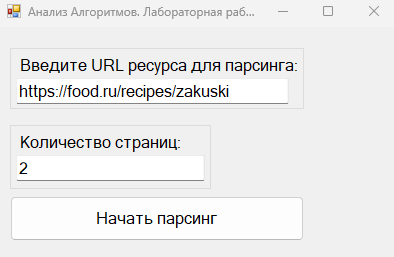
\includegraphics[scale=0.8]{img/1-interface.png}
	\caption{Ввод данных в интерфейс приложения}
	\label{fig:1-prog}
\end{figure}
\begin{figure}[h]
	\centering
	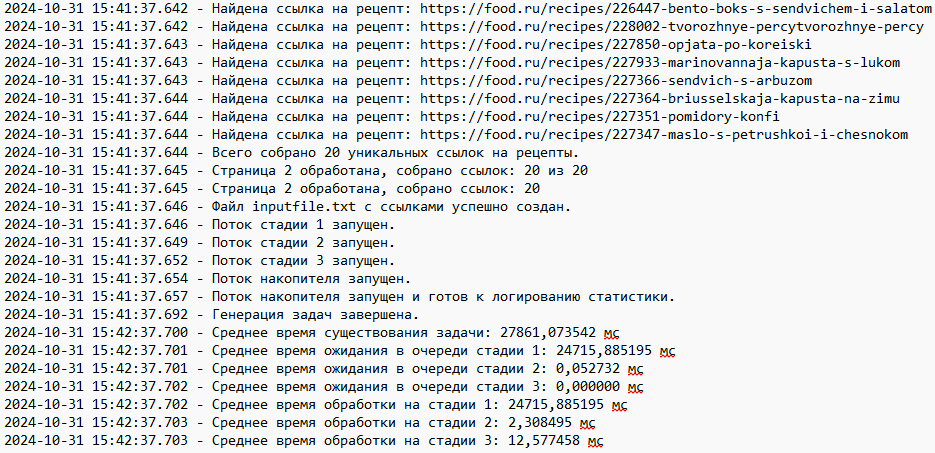
\includegraphics[scale=0.5]{img/3-logmain.png}
	\caption{Сообщения о ходе выполнения парсинга}
	\label{fig:2-prog}
\end{figure}
\begin{figure}[h]
	\centering
	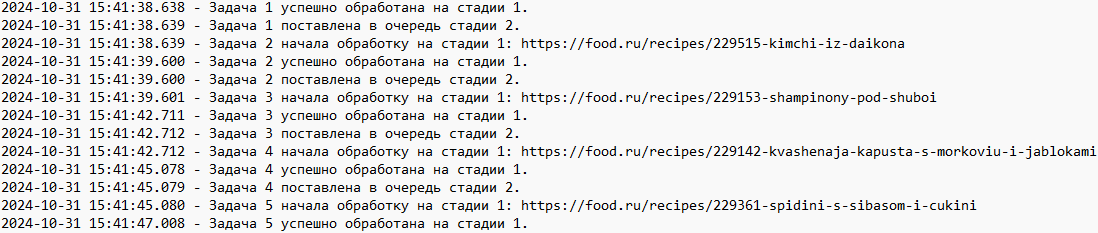
\includegraphics[scale=0.5]{img/4-log1.png}
	\caption{Сообщения о ходе выполнения стадии 1}
	\label{fig:3-prog}
\end{figure}
\begin{figure}[h]
	\centering
	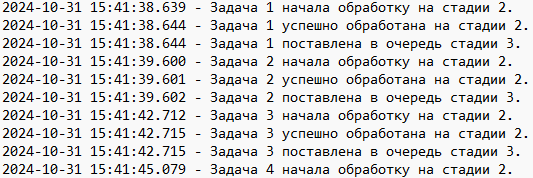
\includegraphics[scale=0.8]{img/5-log2.png}
	\caption{Сообщения о ходе выполнения стадии 2}
	\label{fig:4-prog}
\end{figure}
\begin{figure}[h]
	\centering
	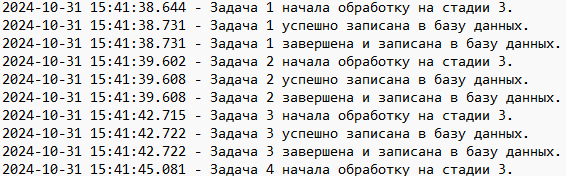
\includegraphics[scale=0.8]{img/6-log3.png}
	\caption{Сообщения о ходе выполнения стадии 3}
	\label{fig:5-prog}
\end{figure}
\begin{figure}[h]
	\centering
	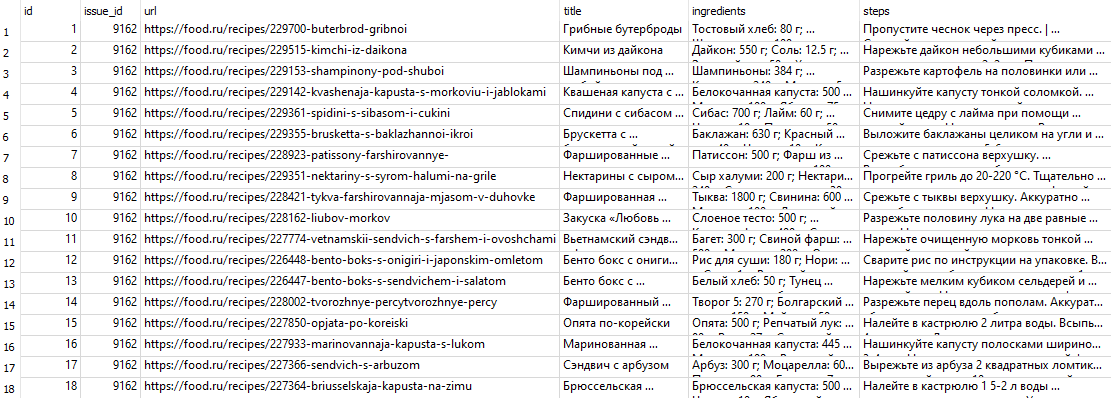
\includegraphics[scale=0.4]{img/2-database.png}
	\caption{Содержимое выходной базы данных}
	\label{fig:6-prog}
\end{figure}

\clearpage

\chapter{Тестирование}

Выполнено тестирование реализованной программы по методологии черного ящика. В таблице~\ref{tbl} представлено описание тестовых случаев. Все тесты пройдены успешно.

\begin{table}[h!]
\begin{center}
\begin{threeparttable}
\caption{Описание тестовых случаев}
\captionsetup{justification=raggedright, singlelinecheck=false}
\label{tbl}
\begin{tabular}{|c|p{6cm}|p{6cm}|c|}
    \hline 
    \textbf{№} & \textbf{Входные данные} & \textbf{Ожидаемый результат} & \textbf{Результат теста} \\
    \hline 
    1 & Пустой базовый URL & Вывод сообщения об ошибке, запрос корректного URL & Пройден \\
    \hline 
    2 & Некорректный базовый URL (без протокола) & Вывод сообщения об ошибке, запрос корректного абсолютного URL & Пройден \\
    \hline 
    3 & Отключенное интернет-соединение & Вывод сообщений об ошибках при загрузке страниц & Пройден \\
    \hline 
    4 & Корректный базовый URL, 1 страница & Успешная загрузка рецептов со страницы, сохранение в \texttt{recipes.db} & Пройден \\
    \hline 
    5 & Корректный базовый URL, 5 страниц & Успешная загрузка рецептов из 5 страниц, сохранение в \texttt{recipes.db} & Пройден \\
    \hline 
    6 & Корректный URL, 0 страниц & Вывод сообщения об ошибке, запрос корректного числа страниц & Пройден \\
    \hline 
    7 & Корректный URL, отрицательное число страниц & Вывод сообщения об ошибке, запрос корректного числа страниц & Пройден \\
    \hline 
\end{tabular}
\end{threeparttable}
\end{center}
\end{table}

\clearpage

\chapter{Описание исследования}

В ходе исследования требуется сформировать лог обработки задач. В таблицах~\ref{1-tb} ---~\ref{4-tb} приведены фрагменты лога обработки. 

\begin{table}[h!]
\begin{center}
\begin{threeparttable}
\caption{Общий лог}
\captionsetup{justification=raggedright, singlelinecheck=false}
\label{1-tb}
\begin{tabular}{|c|p{10cm}|}
    \hline
    \textbf{Время} & \textbf{Статус} \\
    \hline
    2024-10-31 17:22:05.967 & Поток стадии 1 запущен. \\
    2024-10-31 17:22:05.970 & Поток стадии 2 запущен. \\
    2024-10-31 17:22:05.972 & Поток стадии 3 запущен. \\
    2024-10-31 17:22:05.975 & Поток накопителя запущен. \\
    2024-10-31 17:22:05.978 & Поток накопителя готов к логированию статистики. \\
    2024-10-31 17:22:06.001 & Генерация задач завершена. \\
    2024-10-31 17:23:05.999 & Среднее t существования задачи: 32269,128355 мс \\
    2024-10-31 17:23:05.999 & Среднее t ожидания в очереди стадии 1: 26951,583527 мс \\
    2024-10-31 17:23:06.000 & Среднее t ожидания в очереди стадии 2: 0,000000 мс \\
    2024-10-31 17:23:06.000 & Среднее t ожидания в очереди стадии 3: 0,090936 мс \\
    2024-10-31 17:23:06.000 & Среднее t обработки на стадии 1: 26951,583527 мс \\
    2024-10-31 17:23:06.001 & Среднее t обработки на стадии 2: 3,180491 мс \\
    2024-10-31 17:23:06.001 & Среднее t обработки на стадии 3: 7,464700 мс \\
    \hline
\end{tabular}
\end{threeparttable}
\end{center}
\end{table}

\begin{table}[h!]
\begin{center}
\begin{threeparttable}
\caption{Лог стадии 1}
\captionsetup{justification=raggedright, singlelinecheck=false}
\label{2-tb}
\begin{tabular}{|c|p{10cm}|}
    \hline
    \textbf{Время} & \textbf{Статус} \\
    \hline
    2024-10-31 17:22:13.079 & Задача 2 начала обработку на стадии 1: (ссылка) \\
    2024-10-31 17:22:17.636 & Задача 2 успешно обработана на стадии 1. \\
    2024-10-31 17:22:17.636 & Задача 2 поставлена в очередь стадии 2. \\
    2024-10-31 17:22:17.637 & Задача 3 начала обработку на стадии 1: (ссылка) \\
    2024-10-31 17:22:23.061 & Задача 3 успешно обработана на стадии 1. \\
    2024-10-31 17:22:23.062 & Задача 3 поставлена в очередь стадии 2. \\
    2024-10-31 17:22:23.062 & Задача 4 начала обработку на стадии 1: (ссылка) \\
    \hline
\end{tabular}
\end{threeparttable}
\end{center}
\end{table}

\begin{table}[h!]
\begin{center}
\begin{threeparttable}
\caption{Лог стадии 2}
\captionsetup{justification=raggedright, singlelinecheck=false}
\label{3-tb}
\begin{tabular}{|c|p{10cm}|}
    \hline
    \textbf{Время} & \textbf{Статус} \\
    \hline
    2024-10-31 17:22:13.082 & Задача 1 поставлена в очередь стадии 3. \\
    2024-10-31 17:22:17.636 & Задача 2 начала обработку на стадии 2. \\
    2024-10-31 17:22:17.638 & Задача 2 успешно обработана на стадии 2. \\
    2024-10-31 17:22:17.638 & Задача 2 поставлена в очередь стадии 3. \\
    2024-10-31 17:22:23.062 & Задача 3 начала обработку на стадии 2. \\
    2024-10-31 17:22:23.064 & Задача 3 успешно обработана на стадии 2. \\
    2024-10-31 17:22:23.064 & Задача 3 поставлена в очередь стадии 3. \\
    2024-10-31 17:22:27.787 & Задача 4 начала обработку на стадии 2. \\
    \hline
\end{tabular}
\end{threeparttable}
\end{center}
\end{table}

\begin{table}[h!]
\begin{center}
\begin{threeparttable}
\caption{Лог стадии 3}
\captionsetup{justification=raggedright, singlelinecheck=false}
\label{4-tb}
\begin{tabular}{|c|p{10cm}|}
    \hline
    \textbf{Время} & \textbf{Статус} \\
    \hline
    2024-10-31 17:22:13.095 & Задача 1 завершена и записана в базу данных. \\
    2024-10-31 17:22:17.638 & Задача 2 начала обработку на стадии 3. \\
    2024-10-31 17:22:17.645 & Задача 2 успешно записана в базу данных. \\
    2024-10-31 17:22:17.645 & Задача 2 завершена и записана в базу данных. \\
    2024-10-31 17:22:23.064 & Задача 3 начала обработку на стадии 3. \\
    2024-10-31 17:22:23.070 & Задача 3 успешно записана в базу данных. \\
    2024-10-31 17:22:23.070 & Задача 3 завершена и записана в базу данных. \\
    2024-10-31 17:22:27.789 & Задача 4 начала обработку на стадии 3. \\
    \hline
\end{tabular}
\end{threeparttable}
\end{center}
\end{table}

\clearpage

В результате проведённого исследования было подтверждено, что конвейерная обработка выполняет различные этапы параллельно, обеспечивая более высокую скорость обработки по сравнению с простой последовательной обработкой. Однако, поскольку стадия 1 занимает наибольшее время выполнения, вторые и третьи потоки часто простаивают в ожидании следующих задач. Это свидетельствует о возможности дальнейшего улучшения системы для более эффективного использования ресурсов и повышения общей производительности.
